\section{Simulation results}
\label{simulation}

\subsection{Simulation Environment}

The robot dynamics is simulated by numerically integrating the equations of motion with aerodynamic forces Eq.~\eqref{eq_motion_af} in a custom-made simulator implemented in MATLAB-Simulink. The controller is entirely designed in Simulink and runs at a frequency of $\SI{100}{Hz}$. A fast, inner torque control loop is designed to stabilize the joints velocities $\dot{s}$ towards the reference values generated with Eq. \eqref{eq:optimization_QP}.\looseness=-1

\subsection{Flight Envelope Design}

We designed a flight envelope composed as follows:

\begin{enumerate}
  \item \textit{Scenario 1}: the robot hovers in vertical position, while subject to a wind in the frontal direction that follows the profile depicted in Fig. \ref{fig:hovering_wind}. 
  \item \textit{Scenario 2}: the robot hovers and climbs to gain altitude, then moves forward at around $\SI{11}{m/s}$, in presence of a lateral wind with the profile of Fig. \ref{fig:high_speed_wind}.
\end{enumerate}
%
The wind profiles are composed of a constant wind of $\SI{3}{m/s}$, and wind gusts of different shapes with magnitude of $\SI{10}{m/s}$ and $\SI{15}{m/s}$ \cite{ghoreyshi2018simulation,gu2019design,hamel2019unified}.

\subsection{Control Results for the Hovering Scenario}

\begin{figure}[t]
    \centering
        \subfigure{\label{fig:hovering_wind}
        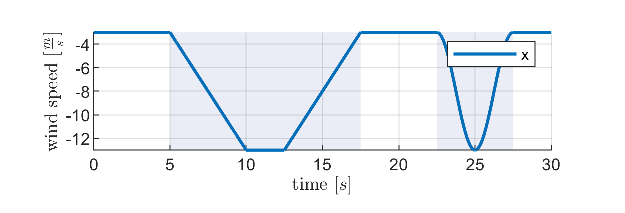
\includegraphics[width=0.97\columnwidth]{./figures/wind_hov.eps}}
        \subfigure{\label{fig:hovering_angMom}
        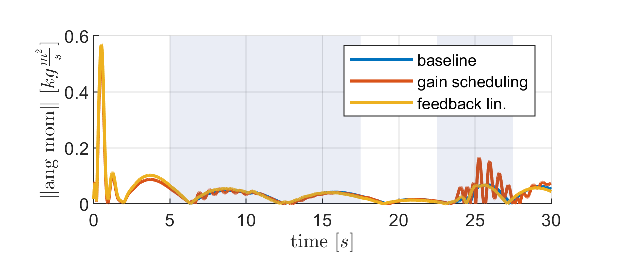
\includegraphics[width=0.97\columnwidth]{./figures/angMom_hov.eps}}
        \subfigure{\label{fig:hovering_linMom}
        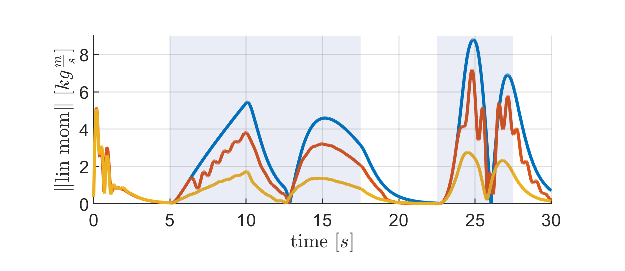
\includegraphics[width=0.97\columnwidth]{./figures/linMom_hov.eps}}
        \subfigure{\label{fig:hovering_com}
        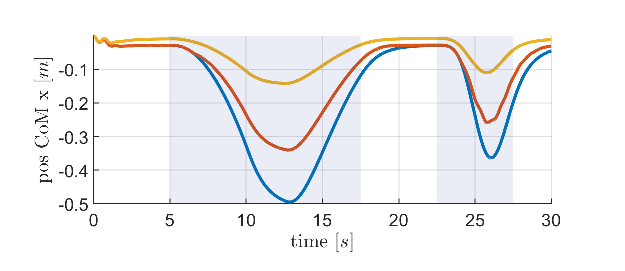
\includegraphics[width=0.97\columnwidth]{./figures/posX_hov.eps}}        
        \caption[]{Hovering scenario. From top to bottom: a) wind profile; b) angular momentum error norm; c) linear momentum error norm; d) center of mass position error in the wind direction.}
        \label{fig:hovering_plots}
\end{figure}

\begin{figure}[t]
    \centering
        \subfigure{\label{fig:high_speed_wind}
        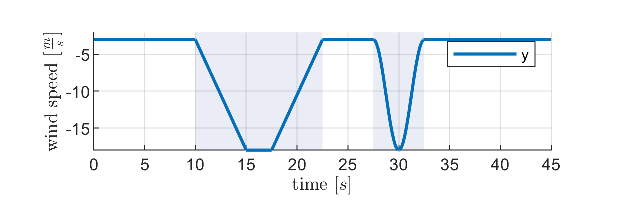
\includegraphics[width=0.97\columnwidth]{./figures/wind_hspe.eps}}
        \subfigure{\label{fig:high_speed_angMom}
        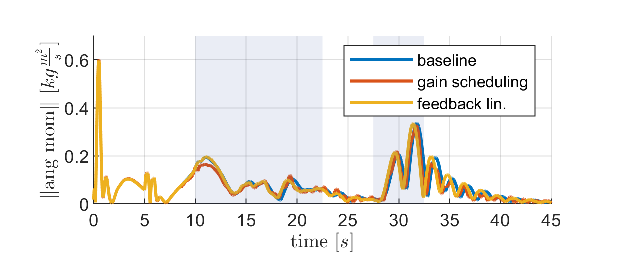
\includegraphics[width=0.97\columnwidth]{./figures/angMom_hspe.eps}}
        \subfigure{\label{fig:high_speed_linMom}
        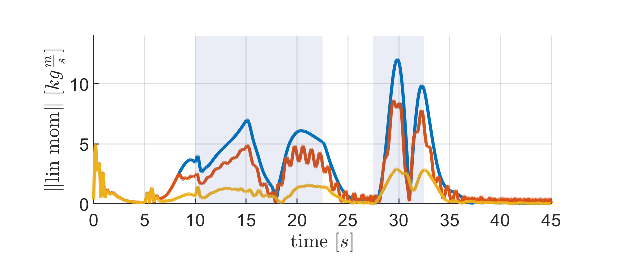
\includegraphics[width=0.97\columnwidth]{./figures/linMom_hspe.eps}}
        \subfigure{\label{fig:high_speed_com}
        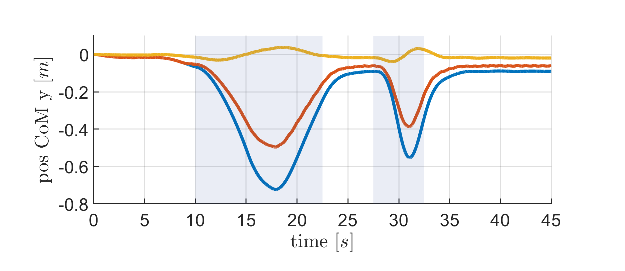
\includegraphics[width=0.97\columnwidth]{./figures/posY_hspe.eps}}        
        \caption[]{High speed flight scenario. From top to bottom: a) wind profile; b) angular momentum error norm; c) linear momentum error norm; d) center of mass position error in the wind direction.}
        \label{fig:high_speed_plots}
\end{figure}

We evaluate the performances of three control strategies: the \emph{baseline} controller of \cite{pucci2017momentum}\cite{nava2018position}, the \emph{feedback linearization} control designed in Sec. \ref{sec:control}, and a third controller that uses \emph{gain scheduling} as described in Sec. \ref{sec:control}. To test the robustness of feedback linearization controller, the aerodynamic force $F_a$ in the control model is computed assuming random noise of $\SI{5}{\%}$ and a calibration error of $\SI{10}{\%}$ on both $\alpha$ and $\beta$ angles.

Simulation results for the hovering scenario are presented in Fig.~\ref{fig:hovering_plots}, where we focused on the linear and angular momentum error norm and center of mass position error. With baseline controller, the center of mass error along the wind direction has peaks of $\SI{50}{cm}$ and $\SI{35}{cm}$ in correspondence of the wind gusts (shaded area), which are reduced by $\SI{33}{\%}$ when the gain scheduling control is used and by $\SI{71}{\%}$ for the feedback linearization control. The linear momentum error also reduces accordingly, while the angular momentum error remains comparable in all three simulations.

\subsection{Control Results for High Speed Flight}
\label{subsec:ctrl-results-aerodyn}

The three controllers are then tested during high speed flight. Fig.~\ref{fig:high_speed_plots} compare their performances in this second scenario: the baseline controller has the worst performances, with peaks errors on the center of mass position of $\SI{75}{cm}$ and $\SI{50}{cm}$. The gain scheduling controller is able to reduce the center of mass peaks error by $\SI{30}{\%}$, while the feedback linearization further reduces the peaks by $\SI{95}{\%}$. Linear and angular momentum errors also behave in accordance with the results already achieved for Scenario 1.